\section{Versuchsaufbau und Versuchsdurchführung}

\begin{flushleft}
    Zusehen sind beide Versuchsaufbauten in Abbildung \ref{Abbildung4} und Abbildung \ref{Abbildung5}.
    Beide bestehen grundsätzlich aus einer Strahlungsquelle, welche sich mit einem Haltungsgerüst und einem Geiger-Müller-Zählrohr, in einem Bleikasten befinden. 
    Das Geiger-Müller-Zählrohr ist dabei mit einem Zählgerät verbunden. 
    Unterscheiden tun sich die Aufbauten durch die Dicke des Bleikastens und die Strahlungsquelle.      
\end{flushleft}

\begin{figure}[H]
    \centering
    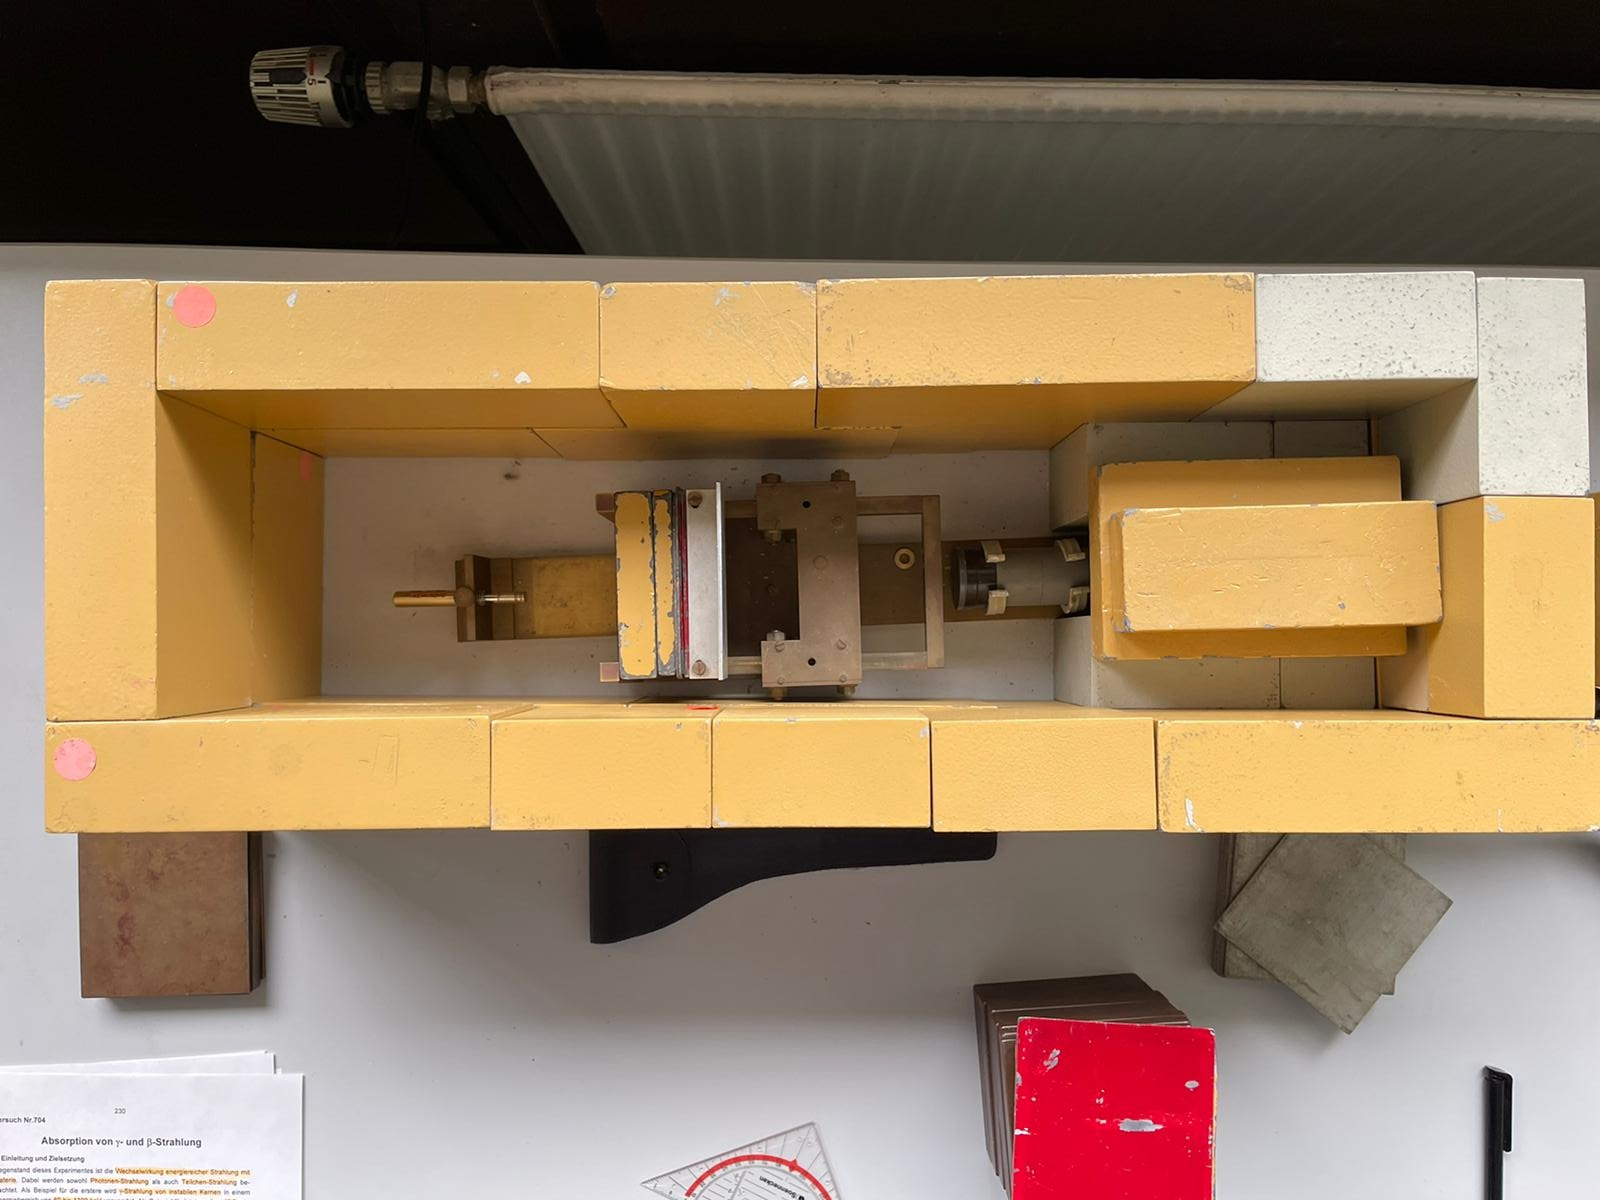
\includegraphics[height=65mm]{bilder/Auf1.jpeg}
    \caption{Versuchsaufbau zum ersten Teil. \label{Abbildung4} }
\end{figure}

\begin{figure}[H]
    \centering
    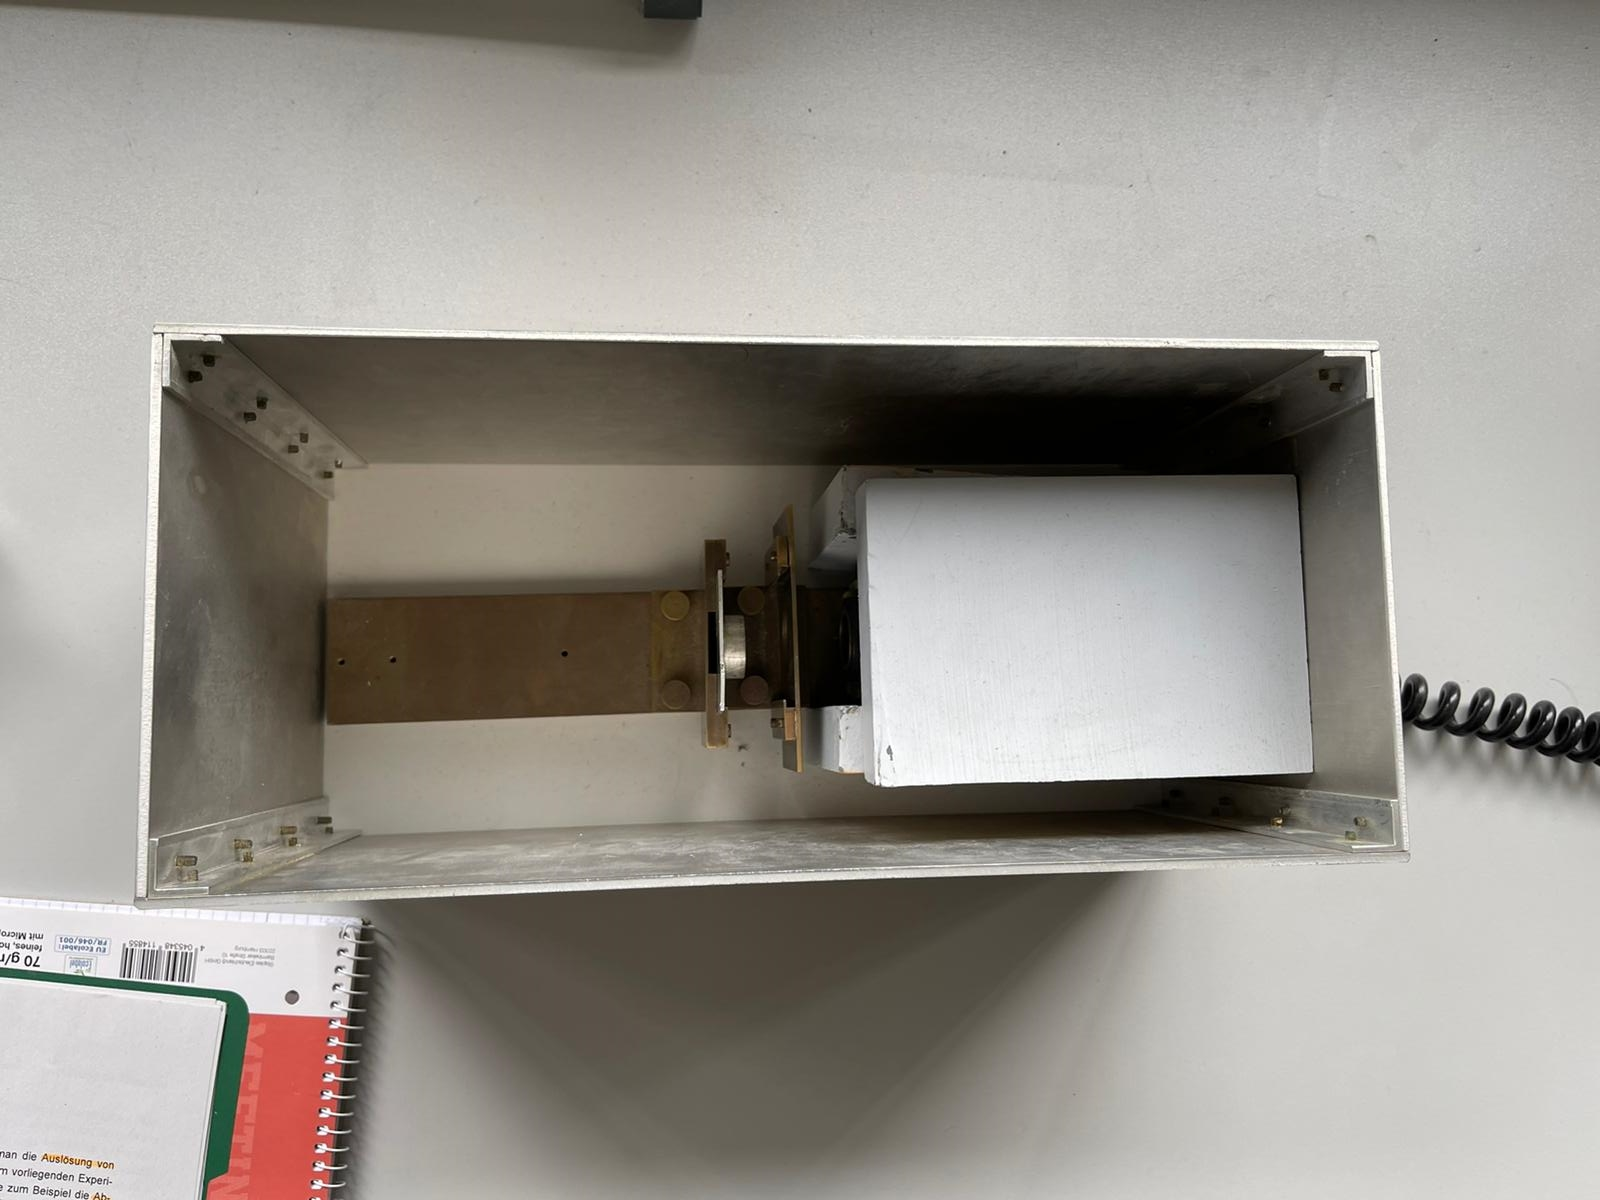
\includegraphics[height=65mm]{bilder/Auf2.jpeg}
    \caption{Versuchsaufbau zum zweiten Teil. \label{Abbildung5} }
\end{figure}

\subsection{Absorption der \textgamma -Strahlung}

\begin{flushleft}
    Der Aufbau wird wie in Abbildung \ref{Abbildung4} zusehen aufgebaut.
    Verwendet wird hierbei Caesium. 
    Zuerst wird die Zählrate des Caesiums ohne Absorber, für $900\,\unit{\second}$, aufgenommen.
    Danach werden für verschiedene dicken, in einem Intervall von 5mm bis 40mm, verschiedene Absorberplatten in die Halterung eingesetzt und die Zählrate erneut gemessen.
    Die Zeit in der die Zählrate gemessen wird ist frei zu wählen, jedoch sollte sie ausreichend lange sein.
    Die Absorberplatten die dabei verwendet werden sind Eisen und Blei. 
    Durchgeführt wird dies für beide Materialien jeweils 12 mal durchgeführt.
\end{flushleft}

\subsection{Absorption der \textbeta -Strahlung}

\begin{flushleft}
    Der Versuch wird wie in Abbildung \ref{Abbildung5} zusehen aufgebaut.
    Verwendet wird hierbei Technetium.
    Wie zuvor wird die Zählrate des Technetiums ohne Absorber, für $900\,\unit{\second}$, aufgenommen.
    Danach werden erneut verschieden dicke Aluminiumabsorber, in einem Intervall von $100\,\unit{\micro\meter}$ bis $482\,\unit{\micro\meter}$, in die Halterung eingesetzt und die Zählrate erneut gemessen.
    Zu Anfang wird die Zählrate nach $100\,\unit{\second}$ aufgenommen, wobei nach jeder Messung die zeit um $15\,\unit{\second}$ verlängert wird. 
    Dies wird für 11 verschiedene Dicken wiederholt.
\end{flushleft}